\documentclass{article}

% packages
\usepackage{amsmath, amsthm, thmtools, amsfonts, amssymb, luacode, catchfile, tikzducks, hyperref, ifthen}
\ifcsname c@kobocompile\endcsname
	\usepackage[a5paper, total={1072pt, 1448pt}, margin=10pt, includeheadfoot]{geometry} % set page margins
\else
	\usepackage[a4paper, margin=50pt, includeheadfoot]{geometry}
\fi
\usepackage[shortlabels]{enumitem}
\usepackage[skip=3pt, indent=0pt]{parskip}

% language
\usepackage[bidi=basic, layout=tabular, provide=*]{babel}
\ifcsname c@english\endcsname
	\babelprovide[main, import]{english}
\else
	\babelprovide[main, import]{hebrew}
	\babelprovide{rl}
\fi
%\babelfont{rm}{Libertinus Serif}
\babelfont{rm}[Renderer=Harfbuzz]{Libertinus Serif}
\babelfont{sf}{Libertinus Sans}
\babelfont{tt}{Libertinus Mono}

% style
\AddToHook{cmd/section/before}{\clearpage}	% Add line break before section
\linespread{1.3}
\setcounter{secnumdepth}{0}		% Remove default number tags from sections, this won't do well with theorems
\AtBeginDocument{\setlength{\belowdisplayskip}{3pt}}
\AtBeginDocument{\setlength{\abovedisplayskip}{3pt}}
\graphicspath{ {../images/} }

% operators
\DeclareMathOperator\cis{cis}
\DeclareMathOperator\Sp{Sp}
\DeclareMathOperator\tr{tr}
\DeclareMathOperator\im{Im}
\DeclareMathOperator\re{Re}
\DeclareMathOperator\diag{diag}
\DeclareMathOperator*\lowlim{\underline{lim}}
\DeclareMathOperator*\uplim{\overline{lim}}
\DeclareMathOperator\rng{rng}
\DeclareMathOperator\Sym{Sym}
\DeclareMathOperator\Arg{Arg}
\DeclareMathOperator\Log{Log}
\DeclareMathOperator\dom{dom}
\DeclareMathOperator\supp{Supp}
\DeclareMathOperator\var{Var}
\DeclareMathOperator\cov{Cov}

% commands
%\renewcommand\qedsymbol{\textbf{מש''ל}}
%\renewcommand\qedsymbol{\fbox{\emoji{lizard}}}
\newcommand{\Aa}[0]{\mathcal{A}}
\newcommand{\Bb}[0]{\mathcal{B}}
\newcommand{\CC}[0]{\mathbb{C}}
\newcommand{\Cc}[0]{\mathcal{C}}
\newcommand{\EE}[0]{\mathbb{E}}
\newcommand{\FF}[0]{\mathbb{F}}
\newcommand{\Ff}[0]{\mathcal{F}}
\newcommand{\Ii}[0]{\mathcal{I}}
\newcommand{\Gg}[0]{\mathcal{G}}
\newcommand{\Ll}[0]{\mathcal{L}}
\newcommand{\Mm}[0]{\mathcal{M}}
\newcommand{\NN}[0]{\mathbb{N}}
\newcommand{\Nn}[0]{\mathcal{N}}
\newcommand{\PP}[0]{\mathbb{P}}
\newcommand{\Pp}[0]{\mathcal{P}}
\newcommand{\QQ}[0]{\mathbb{Q}}
\newcommand{\RR}[0]{\mathbb{R}}
\newcommand{\Rr}[0]{\mathcal{R}}
\newcommand{\Ss}[0]{\mathcal{S}}
\newcommand{\TT}[0]{\mathbb{T}}
\newcommand{\Uu}[0]{\mathcal{U}}
\newcommand{\Vv}[0]{\mathcal{V}}
\newcommand{\Ww}[0]{\mathcal{W}}
\newcommand{\ZZ}[0]{\mathbb{Z}}
\newcommand{\acts}[0]{\circlearrowright}
\newcommand{\explain}[2] {
	\begin{flalign*}
		 && \text{#2} && \text{#1}
	\end{flalign*}
}
\newcommand{\maketitleprint}[0]{ \begin{center}
	%\begin{tikzpicture}[scale=3]
	%	\duck[graduate=gray!20!black, tassel=red!70!black]
	%\end{tikzpicture}	
	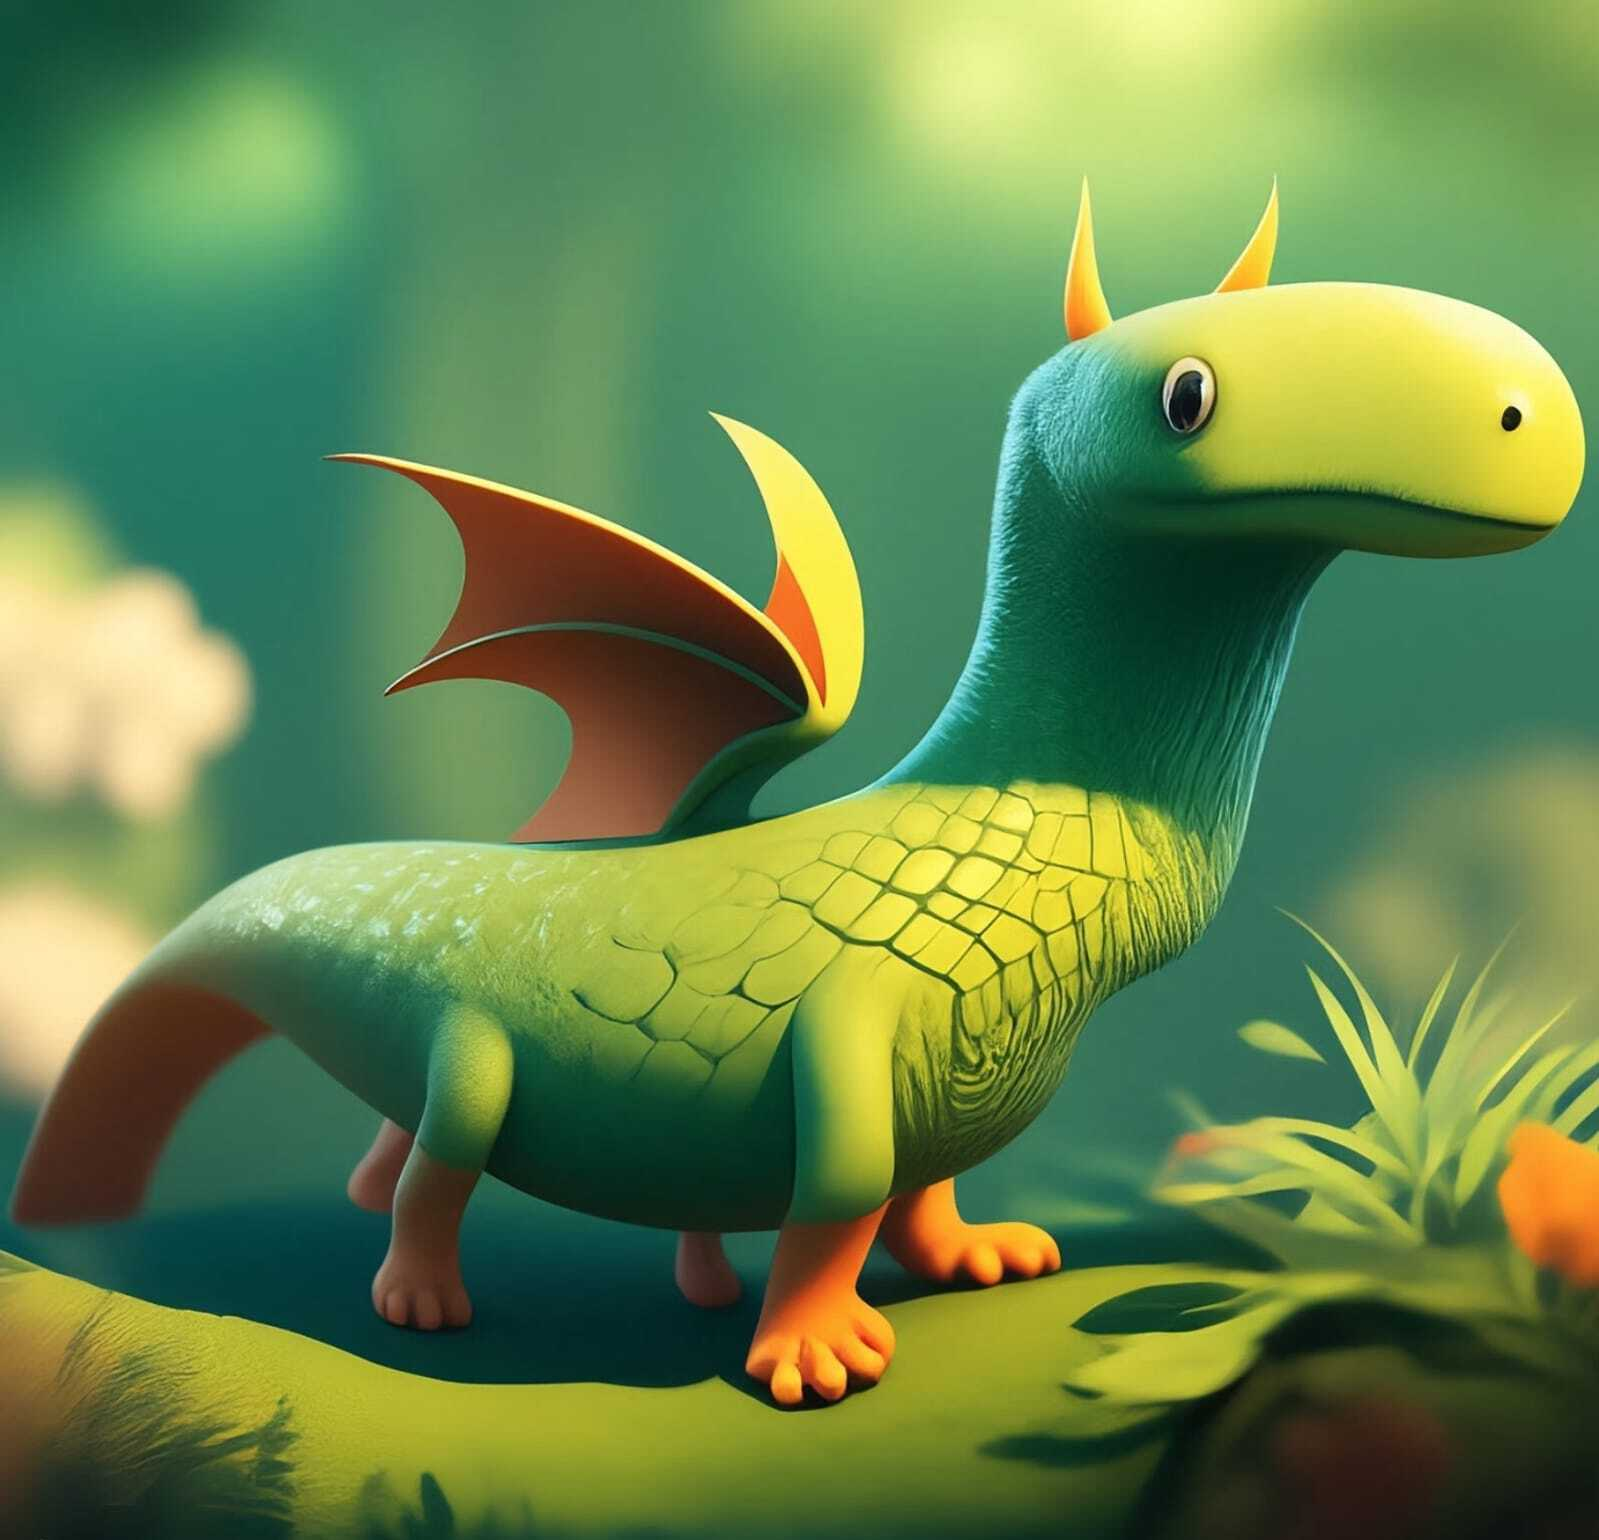
\includegraphics[width=6cm]{cover}
\end{center}
}

% theorem commands
\newtheoremstyle{c_remark}
	{}	% Space above
	{}	% Space below
	{}% Body font
	{}	% Indent amount
	{\bfseries}	% Theorem head font
	{}	% Punctuation after theorem head
	{.5em}	% Space after theorem head
	{\thmname{#1}\thmnumber{ #2}\thmnote{ \normalfont{\text{(#3)}}}}	% head content
\newtheoremstyle{c_definition}
	{3pt}	% Space above
	{3pt}	% Space below
	{}% Body font
	{}	% Indent amount
	{\bfseries}	% Theorem head font
	{}	% Punctuation after theorem head
	{.5em}	% Space after theorem head
	{\thmname{#1}\thmnumber{ #2}\thmnote{ \normalfont{\text{(#3)}}}}	% head content
\newtheoremstyle{c_plain}
	{3pt}	% Space above
	{3pt}	% Space below
	{\itshape}% Body font
	{}	% Indent amount
	{\bfseries}	% Theorem head font
	{}	% Punctuation after theorem head
	{.5em}	% Space after theorem head
	{\thmname{#1}\thmnumber{ #2}\thmnote{ \text{(#3)}}}	% head content

\ifcsname c@english\endcsname
	\theoremstyle{plain}
	\newtheorem{theorem}{Theorem}[section]
	\newtheorem{lemma}[theorem]{Lemma}
	\newtheorem{proposition}[theorem]{Proposition}
	\newtheorem*{proposition*}{Proposition}
	%\newtheorem{corollary}[theorem]{אין חלופה עברית}

	\theoremstyle{definition}
	\newtheorem{definition}[theorem]{Definition}
	\newtheorem*{definition*}{Definition}
	\newtheorem{example}{Example}[section]
	\newtheorem{exercise}{Exercise}[section]

	\theoremstyle{remark}
	\newtheorem*{remark}{Remark}
	\newtheorem*{solution}{Solution}
	\newtheorem{conclusion}[theorem]{Conclusion}
	\newtheorem{notation}[theorem]{Notation}
\else
	\theoremstyle{c_plain}
	\newtheorem{theorem}{משפט}[section]
	\newtheorem{lemma}[theorem]{למה}
	\newtheorem{proposition}[theorem]{טענה}
	\newtheorem*{proposition*}{טענה}
	%\newtheorem{corollary}[theorem]{אין חלופה עברית}

	\theoremstyle{c_definition}
	\newtheorem{definition}[theorem]{הגדרה}
	\newtheorem*{definition*}{הגדרה}
	\newtheorem{example}{דוגמה}[section]
	\newtheorem{exercise}{תרגיל}[section]

	\theoremstyle{c_remark}
	\newtheorem*{remark}{הערה}
	\newtheorem*{solution}{פתרון}
	\newtheorem{conclusion}[theorem]{מסקנה}
	\newtheorem{notation}[theorem]{סימון}
\fi

% Questions related commands
\newcounter{question}
\setcounter{question}{1}
\newcounter{sub_question}
\setcounter{sub_question}{1}

\ifcsname c@english\endcsname
	\newcommand{\question}[1][0]{
		\ifthenelse{#1 = 0}{}{\setcounter{question}{#1}}
		\section{Question \arabic{question}}
		\addtocounter{question}{1}
		\setcounter{sub_question}{1}
	}

	\newcommand{\subquestion}[1][0]{
		\ifthenelse{#1 = 0}{}{\setcounter{sub_question}{#1}}
		\subsection{Part \alph{sub_question}}
		\addtocounter{sub_question}{1}
	}
\else
	\newcommand{\question}[1][0]{
		\ifthenelse{#1 = 0}{}{\setcounter{question}{#1}}
		\section{שאלה \arabic{question}}
		\addtocounter{question}{1}
		\setcounter{sub_question}{1}
	}

	\newcommand{\subquestion}[1][0]{
		\ifthenelse{#1 = 0}{}{\setcounter{sub_question}{#1}}
		\subsection{סעיף \localecounter{letters.gershayim}{sub_question}}
		\addtocounter{sub_question}{1}
	}
\fi

% import lua and start of document
\directlua{common = require ('../common')}

\GetEnv{AUTHOR}

% headers
\author{\AUTHOR}
\date\today

\title{פתרון מטלה 09 --- מבנים אלגבריים 1 (80445)}

\begin{document}
\maketitle
\maketitleprint{}

\Question{}
תהי $G$ חבורה נילפוטנטית.

\Subquestion{}
נוכיח שכל $H \le G$ תת־חבורה היא גם נילפוטנטית.
\begin{proof}
	נניח כי $G$ היא $r$־נילפוטנטית, ונגדיר $\{e\} = Z_0 \triangleleft Z_1 \triangleleft \dots \triangleleft Z_r = G$ הסדרה הנורמלית הנוצרת על־ידי הרכיבים הנילפוטנטיים. \\*
	ממשפט האיזומורפיזם השני נקבל כי $Z_i \cap H \triangleleft H$ לכל $0 \le i \le r$. \\*
	כך נקבל כי $Z(G/Z_i) \simeq Z_{i + 1} / Z_i$ ולכן עלינו להוכיח כי $Z(H / (Z_i \cap H)) \simeq (H \cap Z_{i + 1}) / (H \cap Z_i)$. \\*
	אני לא יודע.
\end{proof}

\Subquestion{}
נוכיח כי לכל $N \triangleleft G$, המנה $G / N$ היא נילפוטנטית.
\begin{proof}
	לא יודע.
\end{proof}

\Question{}
תהי $G$ חבורהה נילפוטנטית סופית.

\Subquestion{}
נוכיח כי לכל $m \mid |G|$ קיימת תת־חבורה $H \le G$ כך ש־$|H| = m$.
\begin{proof}
	אנו יודעים כי קיימת תת־חבורה $p$־סילו יחידה ונורמלית לכל $p$ ואנו יודעים כי גם $G$ היא מכפלה ישרה של חבורות $p$ אלה. \\*
	ידוע גם כי קיימת תת־חבורה מכל סדר חזקת $p$ קטן או שווה לחזקה המקסימלית, ולכן אם ניקח את הפירוק של $m$ לראשוניים, מהעובדה שהוא מחלק את $|G|$ נוכל לקבוע כי לכל $p^r \mid m$ קיימת תת־חבורה בגודל זה ל־$G$. \\*
	נשתמש בעובדה שהיא איזומורפית למכפלה ישרה ונכפול את תת־החבורות האלו בגדלים ראשוניים מקסימליים המחלקים את $m$ ונקבל תת־חבורה $H$ כך שגודלה הוא בדיוק $m$.
\end{proof}

\Subquestion{}
נוכיח כי לכל $p \mid |G|$ ראשוני, מתקיים גם $p \mid |Z(G)|$.
\begin{proof}
	תהי $P$ חבורת $p$־סילו של $G$, וידוע כי $p \mid |Z(P)|$. \\*
	מהמשפט ש־$G$ איזומורפית למכפלה ישרה של חבורות $p$ נסיק כי קיימת חבורה $H \le G$ כך ש־$G \simeq H \times P$, ומהלמה על מרכזי מכפלה ישרה נסיק $Z(G) \simeq Z(H) \times Z(P)$.
	לכן בפרט גם $|Z(G)| = |Z(H)| \cdot |Z(P)|$ ומצאנו כבר כי $p \mid |Z(P)|$ ולכן נסיק כי גם $p \mid |Z(G)|$.
\end{proof}

\Question{}
יהי $\FF$ שדה. תהי $B_n(\FF) \le GL_n(\FF)$ תת־חבורת המטריצות המשולשיות העליות ו־$U_n(\FF) \le B_n(\FF)$ כאשר האלכסון שקול ל־$I_n$.

\Subquestion{}
נוכיח שהחבורה $U_n(\FF)$ היא נילפוטנטית לכל $n \ge 1$.
\begin{proof}
	נניח ש־$U, A \in U_n(\FF)$, ולכן אנו יודעים כי $U \sim I_n$ ולכן נסיק כי קיימת $M \in GL_n(\FF)$ כך ש־$M U M^{-1} = I_n$. \\*
	עתה נבדוק מתי מתקיימת חילופיות ונקבל
	\[
		A U = U A
		\iff A M^{-1} M = M^{-1} M A
		\iff M A M^{-1} = M A
		\iff
		U = A
	\]
	ולכן נסיק כי $Z(U_n(\FF)) = \{ I_n \}$ בלבד, ומכאן נוכל להסיק ישירות כי מתקיימת נילפוטנטיות.
\end{proof}

\Subquestion{}
נוכיח כי החבורה $B_n(\FF)$ היא לא נילפוטנטית לכל $n \ge 2$.
\begin{proof}
	אילו נעשה תהליך דומה לסעיף הקודם נקבל כי המרכז של $B_n(\FF)$ הוא חבורת המטריצות הסקלריות, נסמן $L_n(\FF) = \{ \lambda I_n \mid \lambda \in \FF, \lambda \ne 0_\FF \}$. \\*
	נגדיר הומומורפיזם $\varphi : B_n(\FF) \to B_n(\FF)$ על־ידי $\varphi(B) = \frac{B}{|B|}$, זהו אכן הומומורפיזם כנביעה מהעובדה שדטרמיננטה היא הומומורפיזם. \\*
	נבחין כי $\forall \lambda I_n \in L_n(\FF) : \varphi(\lambda I_n) = 1 / \lambda^n$.
	ממשפט האיזומורפיזם הראשון נסיק כי $B_n(\FF) / Z(B_n(\FF)) \simeq $ \\*
	לא משנה אני לא יודע.
\end{proof}

\Question{}
יהי $R$ חוג ויהיו $x, y \in R$.
נוכיח או נפריך את הטענות הבאות.

\Subquestion{}
נוכיח ש־$x \cdot 0 = 0 \cdot x = 0$.
\begin{proof}
	מפילוג נקבל
	\[
		0 \cdot x = (1 - 1) \cdot x = 1 \cdot x - 1 \cdot x = 0 = x \cdot 1 - x \cdot 1 = x \cdot 0
	\]
\end{proof}

\Subquestion{}
נוכיח כי $(-1) \cdot x = -x$.
\begin{proof}
	$0 = 0 \cdot x = (1 - 1) \cdot x = x + (-1) \cdot x = 0 \implies x + (-1) \cdot x - x = -x \implies (-1) \cdot x = -x$.
\end{proof}

\Subquestion{}
נסתור את הטענה כי ${(x + y)}^2 = x^2 + 2xy + y^2$ על־ידי דוגמה נגדית.

נבחין כי בעוד $x \cdot x$ חילופי בינו לבין עצמו, וכך גם $y = y$, לא בהכרח $xy = yx$. \\*
נבחן את חוג המטריצות $M_2(\RR)$ ונראה כי
\[
	x = \begin{pmatrix}
		1 & 2 \\
		0 & 3
	\end{pmatrix},
	y = \begin{pmatrix}
		1 & 0 \\
		0 & 2
	\end{pmatrix},
	\qquad
	x y = \begin{pmatrix}
		1 & 4 \\
		0 & 6
	\end{pmatrix},
	y x = \begin{pmatrix}
		1 & 2 \\
		0 & 6
	\end{pmatrix}
\]
ולכן נקבל
\[
	{(x + y)}^2
	= \begin{pmatrix}
		2 & 2 \\
		0 & 6
	\end{pmatrix}^2
	= \begin{pmatrix}
		2 & 16 \\
		0 & 36
	\end{pmatrix}
\]
אבל
\[
	x^2 + 2 xy + y^2
	= \begin{pmatrix}
		1 & 7 \\
		0 & 9
	\end{pmatrix}
	+ \begin{pmatrix}
		2 & 8 \\
		0 & 12
	\end{pmatrix}
	+ \begin{pmatrix}
		1 & 0 \\
		0 & 4
	\end{pmatrix}
	= \begin{pmatrix}
		4 & 15 \\
		0 & 25
	\end{pmatrix}
\]
ואלו כמובן מטריצות שונות.

\Subquestion{}
נסתור את הטענה $xy = 0 \implies x = 0 \lor y = 0$ על־ידי דוגמה נגדית.

נגדיר
\[
	x = y = \begin{pmatrix}
		0 & 1 \\
		0 & 0
	\end{pmatrix}
\]
זוהי כמובן מטריצה נילפוטנטית וידוע כי
\[
	x y
	= \begin{pmatrix}
		0 & 1 \\
		0 & 0
	\end{pmatrix}^2
	= 0
\]
אבל $x, y \ne 0$.

\Subquestion{}
נסתור את הטענה $0 = 1 \implies R = \{ 0 \}$ על־ידי דוגמה נגדית.

נגדיר $R = \ZZ_{/2}$ יחד עם פעולת הכפל הטריוויאלית, דהינו $\forall x, y \in R : x \cdot y = 0$, ולכן נקבל כי $0 \cdot x = x \cdot 0 = 0$ ולכן ההגדרה מקיימת את תכונות החוג. \\*
לעומת זאת, $R \ne \{ 0 \}$.

\Question{}
\Subquestion{}
נוכיח שההעתקה $\varphi : \ZZ \to \ZZ_{/n}$ המוגדרת על־ידי $\varphi(x) = x \mod n$ היא הומומורפיזם חוגים.
\begin{proof}
	יהיו $x, y \in \ZZ$, ונוכל לייצגם על־ידי $x = x' + k n, y = y' + k n$ כאשר $k$ משתנה ו־$0 \le x', y' < n$. \\*
	נקבל כמובן $\varphi(x) = x', \varphi(y) = y'$, ועתה נבחין כי $\varphi(x + y) = \varphi(x' + y') = x' + y' \mod n$. \\*
	כמו כן נקבל גם $\varphi(x y) = \varphi((x' + kn)(y' + kn)) = \varphi(x' y' + n(x'k + y'k + k^2)) = x' y' \mod n$. \\*
	נשאר לראות $\varphi(1) = 1$, ואכן על־פי הגדרה שוויון זה מתקיים לכל $n \ge 1$.
\end{proof}

\Subquestion{}
נוכיח שאם $\FF$ שדה ו־$R$ חוג לא אפס, אז כל הומומורפיזם חוגים $f : \FF \to S$ הוא חד־חד ערכי.
\begin{proof}
	מה זה $S$?
\end{proof}

\Subquestion{}
נוכיח שתת־הקבוצה
\[
	C = \left\{
		\begin{pmatrix}
			a & -b \\
			b & a
		\end{pmatrix}
		\middle|
		a, b \in \RR
	\right\}
	\subseteq M_2(\RR)
\]
היא תת־חוג שאיזומורפי ל־$\CC$.
\begin{proof}
	למעשה כבר נתקלנו בהרצאה (שיעור 7) בקבוצה זו, שם הוכחנו כי היא סגורה לכפל ותת־חבורה ללא אפס, דהינו $I_2 \in C$. \\*
	נותר אם כן לבדוק כי היא חבורה יחד עם פעולת החיבור, אנו יודעים כי $0_2 \in C$, ולכן נבדוק סגירות לחיבור וקיום הופכי בלבד:
	\[
		\begin{pmatrix}
			a & -b \\
			b & a
		\end{pmatrix}
		+
		\begin{pmatrix}
			a' & -b' \\
			b' & a'
		\end{pmatrix}
		= \begin{pmatrix}
			a + a' & -(b + b') \\
			b + b' & a + a'
		\end{pmatrix}
		\in C,
		\qquad
		\begin{pmatrix}
			a & -b \\
			b & a
		\end{pmatrix}
		+
		\begin{pmatrix}
			-a & b \\
			-b & -a
		\end{pmatrix}
		= 0_2
	\]
	ומצאנו כי זהו אכן תת־חוג.

	נבדוק איזומורפיה של $C$ ל־$\CC$. \\*
	נגדיר העתקה  $\varphi : C \to \CC$ המוגדרת על־ידי
	\[
		\varphi( \begin{pmatrix}
			a & -b \\
			b & a
		\end{pmatrix}) = a + bi
	\]
	ונבדוק סגירות לחיבור, כפל ויחידה:
	\[
		\varphi(\begin{pmatrix}
			a & -b \\
			b & a
		\end{pmatrix} + \begin{pmatrix}
			a' & -b' \\
			b' & a'
		\end{pmatrix})
		= (a + a') + (b + b')i,
		\varphi(\begin{pmatrix}
			a & -b \\
			b & a
		\end{pmatrix}) + \varphi(\begin{pmatrix}
			a' & -b' \\
			b' & a'
		\end{pmatrix})
		= a + bi + a' + b'i
		= (a + a') + (b + b')i
	\]
	ומצאנו סגירות לחיבור, בגירות לכפל נמצא באותה הדרך בדיוק תוך שימוש בהוכחה שצויינה לעיל מהרצאה 7, וכמובן על־פי הגדרה
	\[
		\varphi(I_2) = 1 + 0i = 1
	\]
	ומצאנו כי זהו הומומורפיזם חוגים, נותר לראות כי הוא הפיך.
	נגדיר $\varphi^{-1} : \CC \to C$ על־ידי
	\[
		\varphi^{-1}(a + bi)
		= \begin{pmatrix}
			a & -b \\
			b & a
		\end{pmatrix}
	\]
	נוכל לבדוק ישירות על־ידי הצבה ונקבל $\varphi \circ \varphi^{-1} = \varphi^{-1} \circ \varphi = Id$ ונסיק כי שניהם אכן איזומורפיזמים, ולכן $C$ איזומורפי ל־$\CC$.
\end{proof}

\end{document}
